\chapter{Flujo con viscosidad dominante}

	
	\begin{itemize}
		\item Si el término de fuerzas viscosas $\mu\triangle\vec{u}$ no es menospreciable
		en la ecuación de Navier-Stokes, ésta puede ser complicada de resolver.
		\item No existe una solución general de la ecuación de Navier-Stokes.
		\item La razón principal es la no-linealidad impuesta por la aceleración
		convectiva en la interpretación euleriana del flujo.
		\item Solo en el caso de geometrías muy sencillas y flujo lento es posible
		encontrar una solución analítica. En estas configuraciones de flujo,
		se produce de una forma u otra una  \textit{linealización}
		de las ecuaciones de Navier-Stokes.
		\item A parte de estos flujos sencillos, existen multitud de resoluciones
		numéricas con geometrías más complicadas y multitud de datos experimentales.
		\item En este tema de flujo viscoso vamos a estudiar algunos de estos flujos
		sencillos que pueden ser analizados de forma analítica. Estos flujos
		estan caracterizados por un número de Reynolds bajo.
		\item Todos los flujos estudiados serán considerados incompresibles, y no
		tendremos en cuenta otros efectos que pudiesen causar una posible
		variación de la densidad. Es decir, no consideraremos las ecuaciones
		de balance de la energía.
	\end{itemize}

\section{Ecuaciones y condiciones de contorno}

	
	Los flujos de fluidos ideales se caracterizan por que, dado que no
	hay viscosidad, no existe la condición de  \textit{no deslizamiento}
	en contacto con paredes sólidas.
	
			Los flujos de fluidos viscosos han de cumplir esta condición de contorno,
			de forma que 
			\[
			\vec{u}=\vec{u}_{s}
			\]
			en los puntos en contacto con un sólido, donde $\vec{v}_{s}$ es
			la velocidad del sólido. A este tipo de condiciones de contorno se
			le denominan \textcolor{blue}{condiciones de contorno de Dirichlet} %

\begin{center}
	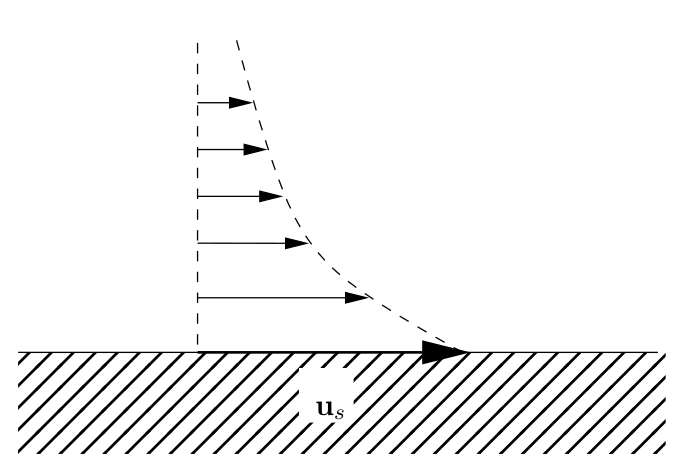
\includegraphics[width=0.5\linewidth]{TeX_files/chapter05-FlujoViscoco/no-slip}
\end{center}


			Otra condición que se ha de cumplir en ciertos puntos es la de esfuerzo
			tangencial nulo. 
			\[
			\tau_{nt}=\mu\dparc{u_{t}}{n}=0.
			\]
			Esta es una \textcolor{blue}{condición de contorno de Neumann}, y
			se cumple, por ejemplo, en planos de simetria y en superficies libres,
			cuando el efecto de la tensión superficial no es importante. %
\begin{center}
	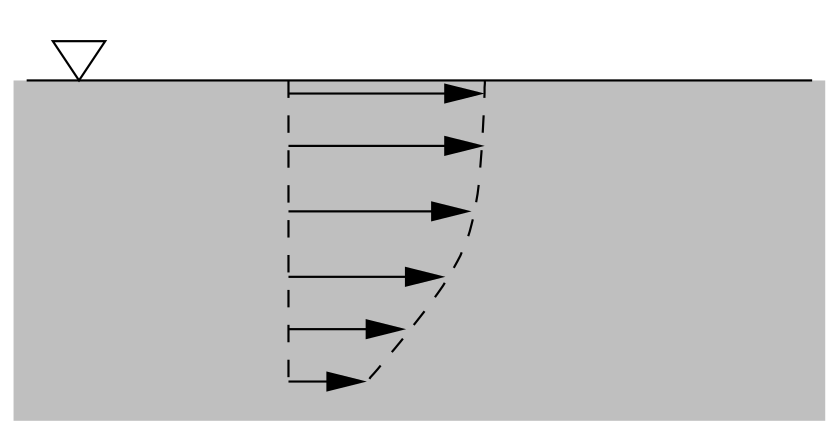
\includegraphics[width=0.5\linewidth]{TeX_files/chapter05-FlujoViscoco/sup_libre}
\end{center}

	
	Todos estos flujos estan descritos por : 
	\begin{itemize}
		\item \textbf{La ecuación de continuidad} 
		
		\begin{equation}
			\vec{\nabla}\cdot\vec{u}=0
		\end{equation}
		
		
		\item \textbf{Las ecuaciones de Navier-Stokes} 
		
		\begin{equation}
			\dparc{\vec{u}}{t}+\left(\vec{u}\cdot\vec{\nabla}\right)\vec{u}=-\dfrac{1}{\rho}\vec{\nabla}p\ +\vec{g}+\dfrac{\mu}{\rho}\triangle\vec{u}
		\end{equation}
		
		
		\item En muchas ocasiones es interesante, o incluso imprescindible, utilizar
		coordenadas polares en flujos bidimensionales y cilíndricas o esféricas
		en flujos tridimensionales.
		\item Las coordenadas esféricas no serán usadas en el presente curso. Las
		ecuaciones de continuidad y Navier-Stokes en coordenadas cilíndricas
		serán vistas en la siguiente sesión.
	\end{itemize}

\section{Flujo entre placas planas paralelas}
	
	\subsection{Flujo entre placas planas paralelas con movimiento relativo
	}
	
	\begin{center}
		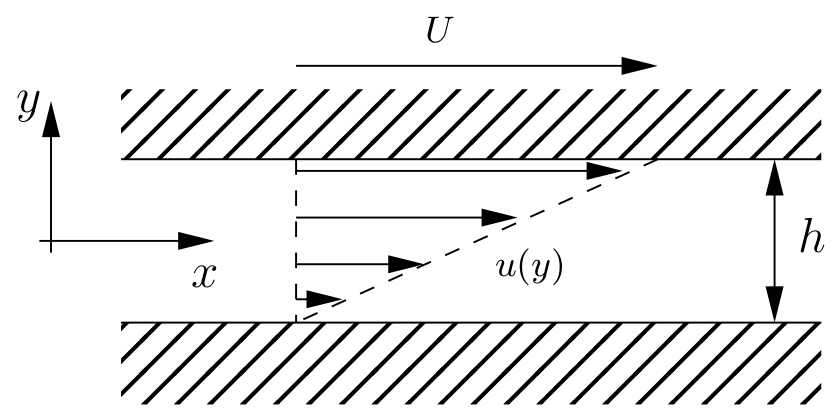
\includegraphics[width=0.5\linewidth]{TeX_files/chapter05-FlujoViscoco/placas1}
	\end{center}
	
			Si las placas son muy grandes en comparación con $h$, el flujo sólo
			tiene dirección $x$, $v=w=0$. El flujo es bidimensional, 
			
			\begin{equation}
				\dparc{}{z}=0
			\end{equation}
			
		
	
	Consideraremos que no hay ningún gradiente de presión, el flujo es
	estacionario, y no afecta la gravedad.
	
	La ecuación de continuidad es 
	
\begin{equation}
		\dparc{u}{x}+\dparc{v}{y}+\dparc{w}{z}=0\,\Rightarrow\,\dparc{u}{x}=0
\end{equation}
	
	, es decir, la velocidad $u$ sólo puede depender de $y$.
	
	Sólo hay una ecuación de Navier-Stokes, la correpondiente a $u$,
	\[
	\underbrace{\dparc{u}{t}}_{\binom{=0}{\text{(est.)}}}+\underbrace{u\dparc{u}{x}}_{\binom{=0}{u(y)}}+\underbrace{v\dparc{u}{y}}_{\binom{=0}{v=0}}=-\underbrace{\frac{1}{\rho}\dparc{p}{x}}_{\binom{=0}{\text{no}\,\vec{\nabla}p}}+\frac{\mu}{\rho}\Bigl(\underbrace{\dparcsec{u}{x}}_{\binom{=0}{u(y)}}+\dparcsec{u}{y}\Bigr)
	\]
	que se reduce a 
	\[
	\derivsec{u}{y}=0\,\Rightarrow\,u=C_{1}y+C_{2}.
	\]
	
	Aplicando las condiciones de contorno \textrm{$u=U\,\text{en}\,y=\frac{h}{2}$
		y $u=0\,\text{en}\,y=-\frac{h}{2}$,} se obtiene 
	\[
	\left.\begin{array}{l}
		U=C_{1}\left(\dfrac{h}{2}\right)+C_{2}\\
		0=C_{1}\left(-\dfrac{h}{2}\right)+C_{2}
	\end{array}\right\} \,\Rightarrow C_{1}=\dfrac{U}{h}\,;\,C_{2}=\dfrac{U}{2}\;\Rightarrow\;\boxed{u=\frac{U}{h}y+\frac{U}{2}}
	\]
	
	
	\subsection{Flujo entre placas planas fijas con gradiente de presión	}
	
	\begin{center}
		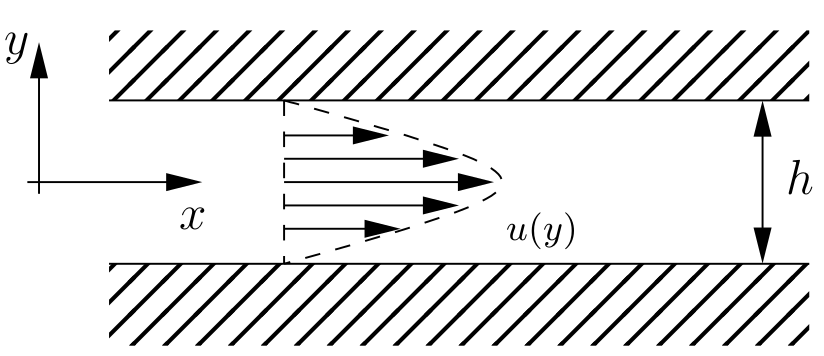
\includegraphics[width=0.5\linewidth]{TeX_files/chapter05-FlujoViscoco/placas2}
	\end{center}
	

			De nuevo el flujo es bidimensional, y $u$ sólo depende de $y$.
			
			La ecuación de Navier-Stokes para $u$ se reduce a 
			
\begin{equation}
				\mu\derivsec{u}{y}=\dparc{p}{x}
\end{equation}
			
			%

	
	Por otro lado, las ecuaciones de Navier-Stokes para las direcciones
	$y$ y $z$ llevan a $\dparc{p}{y}=\dparc{p}{z}=0$. Es decir, $p=p(x)$.
	
	Esto implica que 
	\[
	\mu\derivsec{u}{y}=\deriv{p}{x}=\text{const}<0
	\]
	
	\[
	u(y)=\frac{1}{2\mu}\deriv{p}{x}y^{2}+C_{1}y+C_{2}
	\]

	Las condiciones de contorno son 
\begin{eqnarray*}
	u=0\, & \text{en} & \,y=\frac{h}{2}\\
	u=0\, & \text{en} & \,y=-\frac{h}{2}
\end{eqnarray*}
que llevan a 
\[
\left.\begin{array}{l}
	0=\frac{1}{2\mu}\deriv{p}{x}\left(\frac{h}{2}\right)^{2}+C_{1}\left(\frac{h}{2}\right)+C_{2}\\
	0=\frac{1}{2\mu}\deriv{p}{x}\left(-\frac{h}{2}\right)^{2}+C_{1}\left(-\frac{h}{2}\right)+C_{2}
\end{array}\right\} \Rightarrow\,C_{1}=0\,;\,C_{2}=-\frac{1}{2\mu}\deriv{p}{x}\left(\frac{h}{2}\right)^{2}
\]


\begin{equation}
	\boxed{u(y)=\frac{1}{2\mu}\deriv{p}{x}\left[y^{2}-\left(\frac{h}{2}\right)^{2}\right]}
\end{equation}


Recordemos que la parte anisotrópica del tensor de tensiones (no se
considera la presión) es de la forma
\[
\vec{\vec{\tau}}^{\prime}=2\mu\left(\vec{\nabla}\text{\ensuremath{\vec{u}}}\right)^{S}=\mu\left(\dparc{v}{x}+\dparc{u}{y}\right)\approx\mu\dparc{u}{y}
\]

\subsection*{Actividad 1:}
Calcular la velocidad máxima del flujo y el esfuerzo tangencial en las placas.


\subsection*{Actividad 2:}
Calcular el perfil de velocidades en el caso de dos placas con movimiento
relativo y gradiente de presiones.
	
\section{Ecuaciones de continuidad y Navier-Stokes en coordenadas cilíndricas}

\begin{center}
	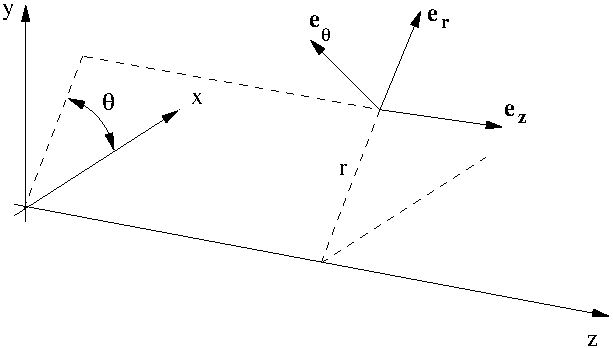
\includegraphics[width=0.5\linewidth]{TeX_files/chapter05-FlujoViscoco/Figures/cilindricas.pdf}
\end{center}

	
	Los operadores diferenciales son definidos de nuevo según :
	
	$\phi$ : escalar ; $\vec{A}$ : vector 
		\[
		\vec{\nabla}\phi=\dparc{\phi}{r}\vec{e}_{r}+\frac{1}{r}\dparc{\phi}{\theta}\vec{e}_{\theta}+\dparc{\phi}{z}\vec{e}_{z}
		\]
		
		\[
		\vec{\nabla}\cdot\vec{A}=\frac{1}{r}\dparc{\phantom{r}}{r}\left(rA_{r}\right)+\frac{1}{r}\dparc{A_{\theta}}{\theta}+\dparc{A_{z}}{z}
		\]
	
		\[
		\begin{aligned}\vec{A}\cdot\vec{\nabla}=A_{r}\dparc{}{r}+\frac{1}{r}A_{\theta}\dparc{}{\theta}+A_{z}\dparc{}{z}\\
			\triangle=\vec{\nabla}^{2}=\frac{1}{r}\dparc{}{r}\left(r\dparc{}{r}\right)+\frac{1}{r^{2}}\dparcsec{}{\theta}+\dparcsec{}{z}\\
			\begin{split}\vec{\nabla}\times\vec{A}=\left(\frac{1}{r}\dparc{A_{z}}{\theta}-\dparc{A_{\theta}}{z}\right)\vec{e}_{r}+\left(\dparc{A_{r}}{\theta}-\dparc{A_{z}}{r}\right)\vec{e}_{\theta}+\left(\frac{1}{r}\dparc{\phantom{r}}{r}\left(rA_{\theta}\right)-\frac{1}{r}\dparc{A_{r}}{\theta}\right)\vec{e}_{z}\end{split}
		\end{aligned}
		\]
	
	El tensor divergencia, en coordenadas cilíndricas, es
	\[
	\nabla\vec{A}=\begin{pmatrix}\dparc{A_{r}}{r} & \dparc{A_{\theta}}{r} & \dparc{A_{z}}{r}\\
		\left(\frac{1}{r}\dparc{A_{r}}{\theta}-\frac{A_{\theta}}{r}\right) & \left(\frac{1}{r}\dparc{A_{\theta}}{\theta}+\frac{A_{r}}{r}\right) & \frac{1}{r}\dparc{A_{z}}{\theta}\\
		\dparc{A_{r}}{z} & \dparc{A_{\theta}}{z} & \dparc{A_{z}}{z}
	\end{pmatrix}
	\]
	
	
	Las ecuaciones en coordenadas cilíndricas son:
	
	\textbf{Continuidad :} 
	
\begin{equation}
		\boxed{\frac{1}{r}\dparc{}{r}(ru_{r})+\frac{1}{r}\dparc{u_{\theta}}{\theta}+\dparc{u_{z}}{z}=0}
\end{equation}
	
	
	\textbf{Navier-Stokes :} {\small{}
		
		\begin{equation}
			\boxed{\begin{array}{ll}
				r\,: & \qquad\dparc{u_{r}}{t}+\bigl(\vec{u}\cdot\vec{\nabla}\bigr)u_{r}-\frac{1}{r}u_{\theta}^{2}=-\frac{1}{\rho}\dparc{p}{r}+g_{r}+\frac{\mu}{\rho}\bigl(\triangle u_{r}-\frac{u_{r}}{r^{2}}-\frac{2}{r^{2}}\dparc{u_{\theta}}{\theta}\bigr)\\
				\theta\,: & \qquad\dparc{u_{\theta}}{t}+\bigl(\vec{u}\cdot\vec{\nabla}\bigr)u_{\theta}+\frac{1}{r}u_{r}u_{\theta}=-\frac{1}{r\rho}\dparc{p}{\theta}+g_{\theta}+\frac{\mu}{\rho}\bigl(\triangle u_{\theta}-\frac{u_{\theta}}{r^{2}}+\frac{2}{r^{2}}\dparc{u_{r}}{\theta}\bigr)\\
				z\,: & \qquad\dparc{u_{z}}{t}+\bigl(\vec{u}\cdot\vec{\nabla}\bigr)u_{z}=-\frac{1}{\rho}\dparc{p}{z}+g_{z}+\frac{\mu}{\rho}\triangle u_{z}
		\end{array}}
		\end{equation}
		
	} 

\section{Flujo de Hagen-Poiseuille}
	
	Consideramos el caso de un flujo en el interior de una tubería infinitamente
	larga, de forma que la velocidad sólo tiene componente en la dirección
	del eje.
	
	Utilizamos coordenadas cilíndricas con el eje $z$ en el eje de la
	tubería.

\begin{center}
	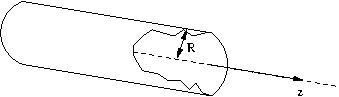
\includegraphics[width=0.5\linewidth]{TeX_files/chapter05-FlujoViscoco/Figures/tubo}
\end{center}

			
			
\begin{equation}
				u_{\theta}=u_{r}=0
\end{equation}
			
			
			Simetría cilíndrica $\rightarrow\dparc{}{\theta}=0$.
			
			Menospreciamos la gravedad y consideramos flujo estacionario.
			
			Ecuación de continuidad: 
			
\begin{equation}
				\dparc{u_{z}}{z}=0\,\Rightarrow\,u_{z}=u_{z}(r)
\end{equation}
			
	
	La ecuación de Navier-Stokes para $u_{z}$ en coordenadas cilíndricas
	es
	\[
	\begin{split}\underbrace{\dparc{u_{z}}{t}}_{\binom{=0}{\text{(estac.)}}}+\underbrace{u_{r}\dparc{u_{z}}{r}}_{\binom{=0}{u_{r}=0}}+\underbrace{u_{\theta}\frac{1}{r}\dparc{u_{z}}{\theta}}_{\binom{=0}{u_{\theta}=0}}+\underbrace{u_{z}\dparc{u_{z}}{z}}_{\binom{=0}{u_{z}=u_{z}(r)}}=\\
		-\frac{1}{\rho}\dparc{p}{z}+\frac{\mu}{\rho}\Bigl[\frac{1}{r}\dparc{}{r}\Bigl(r\dparc{u_{z}}{r}\Bigr)+\underbrace{\frac{1}{r^{2}}\dparcsec{u_{z}}{\theta}}_{\binom{=0}{u_{z}=u_{z}(r)}}+\underbrace{\dparcsec{u_{z}}{z}}_{\binom{=0}{u_{z}=u_{z}(r)}}\Bigr]
	\end{split}
	\]
	
	
\begin{equation}
		\Rightarrow\;\frac{\mu}{r}\deriv{}{r}\left(r\deriv{u_{z}}{r}\right)=\dparc{p}{z}
\end{equation}
	
	
	La ecuación de Navier-Stokes para $u_{r}$ da la condición $\dparc{p}{r}=0$,
	de forma que $p=p(z)$ 
	\[
	\frac{\mu}{r}\deriv{}{r}\left(r\deriv{u_{z}}{r}\right)=\deriv{p}{z}=\text{const}<0
	\]
	
	
	Integrando dos veces esta ecuación, obtenemos
	
	\[
	\deriv{}{r}\left(r\deriv{u_{z}}{r}\right)=\frac{1}{\mu}\deriv{p}{z}r\,\Rightarrow\,\,r\deriv{u_{z}}{r}=\frac{1}{2\mu}\deriv{p}{z}r^{2}+C_{1}
	\]
	
	\[
	\deriv{u_{z}}{r}=\frac{1}{2\mu}\deriv{p}{z}r+\frac{C_{1}}{r}\,\Rightarrow\,u_{z}=\frac{1}{4\mu}\deriv{p}{z}r^{2}+C_{1}\ln r+C_{2}
	\]
	
	Dado que $\ln0$ es una singularidad y en $r=0$ la velocidad del
	flujo ha de ser finita, se tiene que cumplir que $C_{1}=0$.
	
	La condición de contorno $u_{z}=0$ en $r=R$, lleva a 
	\[
	C_{2}=-\frac{1}{4\mu}\deriv{p}{z}R^{2}
	\]
	
	El flujo de Hagen-Poiseuille es, entonces, 
	
\begin{equation}
		\boxed{u_{z}=\left(-\deriv{p}{z}\right)\frac{1}{4\mu}\left(R^{2}-r^{2}\right)}
\end{equation}
	
	
	\subsection*{Actividad 4:}
		Calcular el caudal y el esfuerzo tangencial en las paredes de la
		tubería.

\section{Flujo entre dos cilindros rotatorios concéntricos}
	
	Consideramos el flujo entre dos cilindros concéntricos infinitamente
	largos, de forma que no hay flujo axial ($u_{z}=0,\dparc{}{z}=0$)
	ni efectos de final de tubo.
	
	Los radios de los cilindros en contacto con el fluido son $R_{1}$
	para el interior y $R_{2}$ para el exterior. El cilindro exterior
	está fijo, mientras que el interior rota con una velocidad $\Omega_{1}$.
	Hay simetria cilí ndrica, de forma que no hay variación de la velocidad
	con $\theta$.
	
	La ecuación de continuidad en coordenadas cilíndricas es 
	\[
	\frac{1}{r}\dparc{(ru_{r})}{r}+\underbrace{\frac{1}{r}\dparc{u_{\theta}}{\theta}}_{\binom{=0}{\dparc{}{\theta}=0}}=0\;\Rightarrow\;\frac{1}{r}\deriv{(ru_{r})}{r}=0\;\Rightarrow\;ru_{r}=\text{const.}
	\]
	
	
	Dado que $u_{r}=0$ en $R_{1}$ y en $R_{2}$, se deduce que $u_{r}=0$
	en todo el flujo, y la velocidad es siempre tangencial, $u_{\theta}=u_{\theta}(r)$.
	
	La ecuación de Navier-Stokes para $u_{\theta}$ es, considerando flujo
	estacionario y que no hay gravedad, 
	\[
	\bigl(\vec{u}\cdot\vec{\nabla}\bigr)u_{\theta}+\underbrace{\frac{1}{r}u_{r}u_{\theta}}_{\binom{=0}{u_{r}=0}}=-\underbrace{\frac{1}{r\rho}\dparc{p}{\theta}}_{\binom{=0}{\dparc{}{\theta}=0}}+\frac{\mu}{\rho}\bigl(\triangle u_{\theta}-\frac{u_{\theta}}{r^{2}}+\underbrace{\frac{2}{r^{2}}\dparc{u_{r}}{\theta}}_{\binom{=0}{\dparc{}{\theta}=0}}\bigr)
	\]
	
	La aceleración convectiva también se anula, 
	\[
	\bigl(\vec{u}\cdot\vec{\nabla}\bigr)u_{\theta}=\underbrace{u_{r}\dparc{u_{\theta}}{r}}_{\binom{=0}{u_{r}=0}}+\underbrace{\frac{1}{r}u_{\theta}\dparc{u_{\theta}}{\theta}}_{\binom{=0}{\dparc{}{\theta}=0}}+\underbrace{u_{z}\dparc{u_{\theta}}{z}}_{\binom{=0}{u_{z}=0}}=0
	\]
	y la ecuación se reduce a $\triangle u_{\theta}=\frac{u_{\theta}}{r^{2}}$.
	
	\[
	\triangle u_{\theta}=\frac{1}{r}\dparc{}{r}\left(r\dparc{u_{\theta}}{r}\right)+\underbrace{\frac{1}{r^{2}}\dparcsec{u_{\theta}}{\theta}}_{\binom{=0}{\dparc{}{\theta}=0}}+\underbrace{\dparcsec{u_{\theta}}{z}}_{\binom{=0}{\dparc{}{z}=0}}=\frac{1}{r}\deriv{}{r}\left(r\deriv{u_{\theta}}{r}\right)=\frac{u_{\theta}}{r^{2}}
	\]
	
	La solución general de esta ecuación diferencial ordinaria es 
	\[
	u_{\theta}=C_{1}r+\frac{C_{2}}{r}
	\]
	que, con las condiciones de contorno, {\small{}
		\[
		\left.\begin{array}{ll}
			r=R_{1}\rightarrow & u_{\theta}=\Omega_{1}R_{1}\,\rightarrow\,\Omega_{1}R_{1}=C_{1}R_{1}+\frac{C_{2}}{R_{1}}\\
			r=R_{2}\rightarrow & u_{\theta}=0\,\rightarrow\,0=C_{1}R_{2}+\frac{C_{2}}{R_{2}}
		\end{array}\right\} \Rightarrow\left\{ \begin{array}{l}
			C_{1}=-\dfrac{\Omega_{1}}{\frac{R_{2}^{2}}{R_{1}^{2}}-1}\\
			C_{2}=\dfrac{\Omega_{1}R_{2}^{2}}{\frac{R_{2}^{2}}{R_{1}^{2}}-1}
		\end{array}\right.
		\]
	} 
	\[
	\boxed{u_{\theta}=\frac{\Omega_{1}}{\Bigl(\frac{R_{2}^{2}}{R_{1}^{2}}-1\Bigr)}\Bigl(\frac{R_{2}^{2}}{r}-r\Bigr)}\quad R_{1}\leq r\leq R_{2}
	\]

	
	\subsection*{Actividad 5:}
		Demostrar que el esfuerzo tangencial en el caso de $u_{\theta}(r)$
		es 
		\[
		\tau_{\theta r}=-2\mu\frac{C_{2}}{r^{2}}
		\]

	
	\subsection*{Actividad 6:}
		Cilindro interior: $R_{1}=10\,\text{cm}$ . Exterior: $R_{2}=11\,\text{cm}$.
		Altura: $h=30\,\text{cm}$. Velocidad angular: $\Omega=1200\,\text{rpm}.$
		El fluido tiene una viscosidad $\mu=0.2\,\text{Pa s}$. Calcular el
		momento del rozamiento en el cilindro interior y comparar con el caso
		en que suponíamos una distribución lineal de velocidades.

	
